    
    % PsyConnect Statistics Guide Source Code
    % Copyright (C) 2022 Ho Han Sheng

    % This program is free software: you can redistribute it and/or modify
    % it under the terms of the GNU General Public License as published by
    % the Free Software Foundation, either version 3 of the License, or
    % (at your option) any later version.

    % This program is distributed in the hope that it will be useful,
    % but WITHOUT ANY WARRANTY; without even the implied warranty of
    % MERCHANTABILITY or FITNESS FOR A PARTICULAR PURPOSE.  See the
    % GNU General Public License for more details.

    % You should have received a copy of the GNU General Public License
    % along with this program.  If not, see <https://www.gnu.org/licenses/>.

    \documentclass[a4paper,11pt]{book}
    \usepackage[T1]{fontenc}
    \usepackage[utf8]{inputenc}
    \usepackage{lmodern}
    \usepackage{graphicx}
    \usepackage[english]{babel}
    \usepackage{tikz}
    \usepackage{amsmath,amssymb}
    \usepackage{stackengine}
    \usepackage{stix2}
    \usepackage{stix}
    \usepackage{xcolor}
    \usepackage{array}
    \usepackage{tabulary}
    \usepackage{longtable}
    \usepackage{siunitx}
    \usepackage[style=apa]{biblatex}
    \usepackage{csquotes}
    \usepackage{indentfirst}
    \usepackage{mathtools}
    \usepackage{hyperref}
    
    \addbibresource{bibliography.bib}
    
    \usetikzlibrary{tikzmark,calc,decorations.pathreplacing}
    
    % Colours are nice
    \definecolor{sussblue}{RGB}{0,59,92}
    \definecolor{sussred}{RGB}{218,41,28}
    
    
    % Define new commands
    
    \newcommand\deci[1]{%   <--- Decimal position to right
        \kern-.4ex\stackunder[0.4pt]{$#1$}{$\color{sussred}\acwunderarcarrow$}
    }
    
    \newcommand\decil[1]{%    <--- Decimal position to left
        \kern-.4ex\stackunder[0.4pt]{$#1$}{%
          \reflectbox{$\color{sussred}\kern-.6ex\acwunderarcarrow$}
          }
    }
    
    \tikzset{square arrow below/.style={
        to path={-- ++(0,-.25)  -| (\tikztotarget) \tikztonodes},below,pos=.25}}
        
    \tikzset{square arrow above/.style={
        to path={-- ++(0,.25)  -| (\tikztotarget) \tikztonodes},above,pos=.25}}
    
    
    % 'dedication' environment: To add a dedication paragraph at the start of book %
    
    \newenvironment{dedication}
    {
       \cleardoublepage
       \thispagestyle{empty}
       \vspace*{\stretch{1}}
       \hfill\begin{minipage}[t]{0.66\textwidth}
       \raggedright
    }
    {
       \end{minipage}
       \vspace*{\stretch{3}}
       \clearpage
    }
    
    % Book's title and subtitle
    \title{\Huge \textbf{PsyConnect Statistics Guide}  \\ \huge v0.1}
    % Author
    \author{\textsc{\underline{Ho} Han Sheng}\thanks{\url{https://github.com/ho-han-sheng}}}
    \date{published date}
    
    \begin{document}
    
    \frontmatter
    \maketitle
    
    % Dedication page
    \begin{dedication}
    Dedicated to M, B and BB.
    \end{dedication}
    
    % Auto-generated table of contents, list of figures and list of tables 
    \tableofcontents
    \listoffigures
    \listoftables
    
    \mainmatter
    
    % Preface %
    \chapter*{Preface}
    \markboth{PREFACE}{} % Fixes table of contents header spilling over
    A common aversion faced by psychology undergraduates around the world is the need to study statistics. Given the relative infancy of psychology compared to other hard science fields or even the humanities, it is imperative that we as psychologists are able to read, comprehend and incorporate the most recent research as part of our continuous learning journey. With strong statistical foundations, one would be able to discern sound and rigourous statistical analyses from misleading or erroneous methods used in a fair percentage of psychological research \autocite{Bakker2011}. 
    
    In some universities, the compulsory statistics modules are taught by mathematics professors. This is logical given their area of expertise, although it may further exacerbate the "expert blind spot" effect \autocite{Nathan2003}. As experts, professors perform many abstract and symbolic reasoning steps automatically, "jumping" from one train of thought to another seamlessly as they would perceive. However, as undergraduates attempting to learn these concepts from scratch, it is exceptionally difficult to be able to "see" these connections automatically or even at all. Additionally, as psychology majors, certain "mathematical connections" inculcated in students majoring in fields requiring substantial mathematical foundations (e.g. engineering, computer science, mathematics) would be difficult to develop in short duration. What professors feel is trivial and does not require explicit instruction then, is what leads to students falling through the cracks. 
    
    In the case of my university (Singapore University of Social Sciences), the psychology program is fully part-time. The typical student profile then consists of mid-career switchers, mature adults and others who have gone years since their last interaction with mathematics. Assuming one leaves the education system with a GCE "O" Levels at 16 years old and pursues a non-mathematically heavy diploma in a polytechnic, it would be 6 years (!) before one can enrol in a part-time course with 2 years of working experience at 22 years old. That is akin to spending 6 years in a sedentary lifestyle with minimal exercise, making it difficult to return to a certain level of fitness. 
    
    \section*{What this book is for}
    This book serves to hopefully bridge the gap between expert knowledge and novice learning. Content will first focus on topics expected of students at "O" Levels, following the syllabus document published by the Singapore Examinations and Assessment Board. Afterwards, topics related to or typically required to understand statistical concepts at the undergraduate level will be discussed. 
    
    By attempting to keep technical jargon to a minimum, this book should require minimal effort to comprehend. It would also provide a sort of "warm-up" for students' minds to prepare them to think mathematically, serving as pre-reading before they embark on their statistics modules.
    
    \section*{What this book is for me}
    My handwriting is terrible. When I first started my statistics modules, I needed a way to write my notes such that they were at least legible and easily written (i.e. typed out because I'm lazy). I was already using Notion to develop my own notes for my psychology modules and a quick google bestowed upon me the masterpiece that is \LaTeX{}. Notion allowed me to typeset mathematical formulae with \LaTeX{} commands and what followed was the development of my summary notes that were shared to my fellow psychology peers. 
    
    This book is then a personal project for me to further develop my skills in working with \LaTeX{}, from typesetting everything within the document, learning the uses of various packages (\textsc{TikZ}, \textsc{tabulary}, \textsc{Bib}\LaTeX{} etc.) to creating my own graphics and figures in \LaTeX{}.
    
    
    \section*{About the companion website}
    The website\footnote{\url{https://github.com/ho-han-sheng/psyconnect-statistics-guide}} for this file contains:
    \begin{itemize}
      \item The (freely downlodable) latest version of this document.
      \item The LaTeX source code for this document.
      \item A way to propose amendments through pull requests.
    \end{itemize}
    
    
    \newpage
    \section*{Acknowledgements}
    A special word of thanks goes to 
    \begin{itemize}
    \item The PsyConnect EXCO Team
    \item 
    \end{itemize}
    
    \noindent Ho Han Sheng
    
    
    
    % Start actual book content
    \chapter{Numbers and Algebra}
    
    \section{Numbers and their operations}
    
    \subsection{Number systems}
    
    What do these funny looking letters $\mathbb{R}$, $\mathbb{N}$, $\mathbb{Z}$, $\mathbb{Q}$ mean? These symbols denote which sets a particular number falls under (real, natural, integer etc.). Later on we will look at how these symbols may be used in set theory. Table \ref{tab:Number set notations} on page \pageref{tab:Number set notations} outlines the main terms used. 
    
    \begin{table}[p]
        \centering
        \settowidth\tymin{{Example} + 5pt}
        \setlength\extrarowheight{4pt}
            \begin{tabulary}{\linewidth}{|L|C|J|C|}
                \hline
                \textbf{Set} & \textbf{Symbol} & \textbf{Definition} & \textbf{Example} \\
                \hline \hline
                Natural numbers & $\mathbb{N}$ & Also called counting numbers, these are numbers we use to count items & $1, 2, 3, 4, 5$, \ldots \\
                \hline
                Whole numbers & No official symbol & Includes the set of natural numbers and $0$ & $0, 1, 2, 3, 4, 5$, \ldots \\
                \hline
                Integers & $\mathbb{Z}$ & Consists of whole numbers, their opposites and $0$ & \ldots $,-3, -2, -1,$ $0, 1, 2, 3$, \ldots \\
                \hline
                Rational numbers & $\mathbb{Q}$ & All numbers that can be expressed as a fraction & $44, -\frac{17}{5},$ $0.1\dot{2} = \frac{11}{90}$ \\
                \hline
                Irrational numbers & No official symbol & Numbers that cannot be expressed as a fraction & $\pi, \sqrt{2}, -3\pi,$ Euler's number \\
                \hline
                Real numbers & $\mathbb{R}$ & Encompasses all rational and irrational numbers. Every number that can exist on a typical number line & \ldots $, -5, -\pi, 0,$ $\sqrt{17}, 75$\\
                \hline
                Imaginary numbers & No official symbol & Any real number multiplied by $\sqrt{-1} = i$ & $2i, \pi i, -3i$ \\
                \hline
                Complex numbers & $\mathbb{C}$ & Includes the set of real numbers. Any number that has a real part and imaginary part. & $(2+3i), (\pi - 6i)$ \\
                \hline
            \end{tabulary}
        \caption{Number Set Notations}
        \label{tab:Number set notations}
    \end{table}
    
    \subsection{Less than, greater than or equal to}
    Also called inequality symbols, they are used to represent the relationship between two variables or expressions.
    \medskip
    
    \par The value of \(a\) is less than the value of \(b\):
    \[a < b\]
    
    
    The value of \(a\) is greater than the value of \(b\):
    \[a > b\]
    
    
    The value of \(a\) is less than or equal to the value of \(b\):
    \[a\leq b\]
    
    
    The value of \(a\) is greater than or equal to the value of \(b\):
    \[a\geq b\]
    
    \textbf{Useful Tip:} Imagine the inequality symbol as a crocodile's mouth and that the crocodile prefers eating larger numbers.
    
    \subsection{Approximation and estimation}
    Significant figures refer to the number of digits in a value that are necessary and contribute to the degree of accuracy of the quantity of something. Insufficient significant figures during your calculations can lead to an inaccurate final answer. As a rule of thumb, \emph{five} significant figures are used for intermediate calculations and \emph{three} significant figures are used for your final answer. 
    
    We start by counting the digits from left to right, beginning with the first \emph{non-zero} digit. To round off to \emph{three} significant figures, we have to look at the fourth non-zero digit from the left. 
    
    \[0.0\tikzmark{a}{7}56\tikzmark{e}{9}\]
    
    \[\tikzmark{b}{7}89\tikzmark{f}{0}43.0889\]
    
    \[0.0\tikzmark{c}{4}59\tikzmark{g}{6}0\]
    
    \[\tikzmark{d}{3}00\tikzmark{h}{2}.01\]
    
    \begin{tikzpicture}[remember picture,overlay]
    
    %There's probably a better way to use tikzmarks here but it works so
    % todo align the 1st and 4th labels
    {
    \foreach \Value in {a, b, c, d}
    \draw [<-]
      ([yshift = -2pt, xshift = 3.5pt]pic cs:\Value) node[anchor = south] {} -- ([yshift = -8pt, xshift = 3.5pt]pic cs:\Value) 
      node[anchor=north, inner sep = 0.5pt] {1st};
    
    \foreach \Value in {e, f, g, h}
    \draw [<-]
      ([yshift = -2pt, xshift = 3.5pt]pic cs:\Value) node[anchor = south] {} -- ([yshift = -8pt, xshift = 3.5pt]pic cs:\Value) 
      node[anchor=north, inner sep = 0.5pt] {4th};
    }
    \end{tikzpicture}
    
    The value of this fourth digit determines how we round off the number. If the value of the fourth digit is $\geq5$ then we will add 1 to the third digit. 
    
    % todo align all equations at approx
    
    \[0.075 \tikzmarknode{1a}{6}9 \approx 0.0757\]
    
    \[78 \tikzmarknode{1b}{9}043.0889 \approx 789000\]
    
    \[0.045\tikzmarknode{1c}{9}60 \approx 0.0460\]
    
    \[30\tikzmarknode{1d}{0}2.01 \approx 3000\]
    
    \begin{tikzpicture}[remember picture,overlay]
    
    
    {
    \foreach \Value in {1a, 1c}
    \draw [<-]
      ([yshift = -2pt]pic cs:\Value) node[anchor = south] {} -- ([yshift = -8pt]pic cs:\Value) 
      node[anchor=north, inner sep = 0.5pt] {Add 1};
    
    \foreach \Value in {1b, 1d}
    \draw [<-]
      ([yshift = -2pt]pic cs:\Value) node[anchor = south] {} -- ([yshift = -8pt]pic cs:\Value) 
      node[anchor=north, inner sep = 0.5pt] {Keep value};
    }
    
    \end{tikzpicture}
    
    If the value of the fourth digit is $\leq4$, then we will keep the value of the third digit. Note that the subsequent digits will become 0. For \emph{five} significant figures then, we would look at the sixth non-zero digit from the left.
    
    \pagebreak
    \subsection{Scientific notation}
    Also known as standard form. This is a way to express numbers that are either very large or very small.
    
    \[ A \times 10^n \]
    
    Where $n$ is an integer\footnote{Do you remember what an integer is? Refer back to Table \ref{tab:Number set notations} if you need to.} and $1 \leq A < 10$
    \medskip
    
    The advantage of scientific notation lies in its lack of ambiguity in the number of significant figures. Refer to the number 3000, which is valid for 1, 2, 3 or 4 significant figures. As seen in Table \ref{tab:Decimal and scientific notation}, $3.251 \times 10^{6}$ is clearly 4 significant figures. Some calculators display $\text{\sc{e}}$ in place of $\times 10$. $3.251 \times 10^{6}$ would then appear as $3.251\text{\sc{e}}6$.
    
    \begin{table}[htb]
        \centering
        {\renewcommand{\arraystretch}{1.5}%
        \begin{tabular}{|l|r|}
        \hline
        \textbf{Decimal Notation} & \textbf{Scientific Notation}  \\
        \hline \hline
        3     &   $3 \times 10^{0}$  \\
        \hline
        3000 &   $3 \times 10^{3} $   \\
        \hline
        3251000 & $3.251 \times 10^{6}$   \\
        \hline
        0.02 &  $2 \times 10^{-2}$    \\
        \hline
        0.0000451 & $4.51 \times 10^{-5}$ \\
        \hline
        0.000060075 & $6.0075 \times 10^{-5}$  \\
        \hline
        \end{tabular}}
        \caption{Decimal and Scientific Notation}
        \label{tab:Decimal and scientific notation}
    \end{table}
    
    \textbf{Useful Tip:} $n$ can be thought of as the number of times we move the decimal point left or right\footnote{Only applicable for base 10.}. 
    
    \[ 3.251 \times 10^{6} = 3. \underbrace{\deci{2}\deci{5}\deci{1}\deci{0}\deci{0}\deci{0}}_{6 \:\text{places}} = 3251000 \]
    
    \[ 6.0075 \times 10^{-5} = 0\, \underbrace{\decil{0}\decil{0}\deci{0}\decil{0}\decil{6}}_{5 \: \text{places}}.0075 = 0.000060075 \]
    
    \pagebreak
    \subsection{Indices}
    
    An index (Plural: indices) is the small superscript number that appears above a number. It denotes the number of times that number is multiplied by itself. $10^{4}$ means 10 multiplied by itself 4 times, $10 \times 10 \times 10 \times 10 = 10000$. We can read this as "10 to the power of 4" or "10 raised to the power of 4".
    
    \[ \tikzmarknode{base}{a}^{\tikzmarknode{index}{m}} \]
    
    \begin{tikzpicture}[remember picture,overlay]
    \draw[<-] 
      ([shift={(0pt,-2pt)}]pic cs:base) |- ([shift={(-10pt,-10pt)}]pic cs:base) 
      node[anchor=east] {Base}; 
    \draw[<-] 
      ([shift={(2pt,5pt)}]pic cs:index) node[anchor=north] {} |- ([shift={(10pt,14pt)}]pic cs:index) 
      node[anchor=west] {Index}; 
    \end{tikzpicture}
    
    There exists index laws and rules that allow us to simplify expressions when working with indices.
    
    %%todo align all equations 
    
    \begin{equation}\label{eqn:index law one}
        a^m \times a^n = a^{m+n}
    \end{equation}
    
    \[2^4 + 2^3 = 2^{4+3} = 2^7 = 128\]
    
    \emph{\ref{eqn:index law one}}. If 2 numbers with the same base are multiplied together, the result is equal to the same base raise to the power of the sum of the 2 indices. 
    
    \begin{equation}\label{eqn:index law two}
        (a^m)^n = a^{m\times n}
    \end{equation}
    
    \[ (2^4)^3 = 2^{4 \times 3} = 2^{12} = 4096 \]
    
    \emph{\ref{eqn:index law two}}. If a number $a^m$ is itself raised to another power, the result is equal to the same base raised to the power of the 2 indices multiplied together.
    
    \begin{equation}\label{eqn:index law three}
        \frac{a^m}{a^n} = a^{m-n}
    \end{equation}
    
    \[ \frac{2^5}{2^3} = 2^{5-3} = 2^2 = 4\]
    
    \[ \frac{2^5}{2^3} = 2^5/2^3 \]
    
    \emph{\ref{eqn:index law three}}. The result of the division of 2 indices is equal to the same base raised to the power of the subtraction of the denominator's index from the numerator's index. 
    
    \pagebreak
    \begin{equation}\label{eqn:index law four}
        a^{-m} = \frac{1}{a^m}
    \end{equation}
    
    \[ 2^{-3} = \frac{1}{2^3} \]
    
    \emph{\ref{eqn:index law four}}. The result of a number raised to a negative power is equal to the reciprocal\footnote{The reciprocal of $X = \frac{1}{X}$} of the same number raised to a positive number of the same value. 
    
    \begin{equation}\label{eqn:index law five}
        a^0 = 1
    \end{equation}
    
    \[ 2^0 = 381^0 = 0^0 = 1 \]
    
    \emph{\ref{eqn:index law five}}. Any base raised to the power of 0 will always give a value of 1.
    
    \begin{equation}\label{eqn:index law six}
        a^{\frac{m}{n}} = \sqrt[n]{a^m}
    \end{equation}
    
    \[ 4^{\frac{2}{3}} = \sqrt[3]{4^2} \]
    
    \emph{\ref{eqn:index law six}}. If the index is a fraction, the denominator $n$ indicates the $n\text{th}$ root and the numerator indicates the power to raise the base by. 
    
    \begin{equation}\label{eqn:index law seven}
        a^m \times b^m = ab^m
    \end{equation}
    
    \[ 2^3 \times 4^3 = (2 \times 4)^3 = 8^3 = 512 \]
    
    \emph{\ref{eqn:index law seven}}. The result of the multiplication of 2 numbers with different bases but with the same index is equal to the multiple of both bases raised to the same power. 
    
    \begin{equation}\label{eqn:index law eight}
        a^m / b^m = \frac{a^m}{b^m} = \bigg(\frac{a}{b}\bigg)^m
    \end{equation}
    
    \[ \frac{2^5}{3^5} = \bigg(\frac{2}{3}\bigg)^5 = \frac{32}{243} \]
    
    \emph{\ref{eqn:index law eight}}. The division of 2 numbers with different bases but with the same index yields a result equal to the fraction (or division) of the two bases raised to the same power. 
    
    \section{Percentages}
    
    We frequently deal with percentages in statistics; From deriving the probability of an event occurring from a given proportion to determining our level of significance for hypothesis testing. It is imperative then for us to understand how to work with percentages and how to derive them when required.
    
    \begin{figure} [hb]
        \centering
        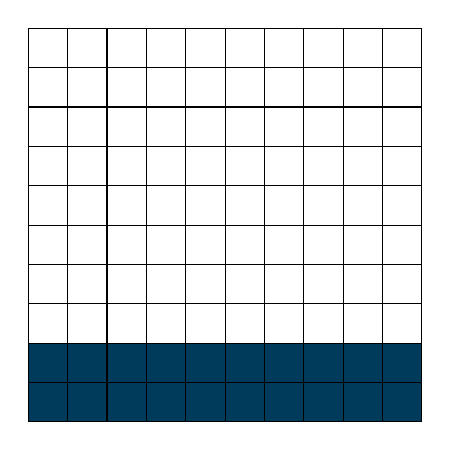
\begin{tikzpicture}
            
            \fill[fill = sussblue, draw = black, step = 5mm] (0,0) rectangle (5,1);
            \draw[step = 5mm] (0,0) grid (5,5);
            
        \end{tikzpicture}
        \caption{20 Shaded Squares out of 100, 20\%}
        \label{fig:20 shade square}
    \end{figure}
    
    The dictionary definition of "percent" is "of each 100" \autocite{dictpercent}. Percentages can also be expressed as fractions or decimals. For example, 20 out of 100 can be expressed as:
    
    % GFI: arrows to denote divide 20 and 100 by 10 to give 2 and 10.
    \[ \frac{\tikzmark{3a}{20}}{\tikzmark{3b}{100}} = \frac{\tikzmark{3c}{2}}{\tikzmark{3d}{10}} = 0.2 = 20\% \]
    
    If the total quantity is not out of 100, we can (1) divide the two quantities to obtain the decimal form of the percentage or (2) multiply the result by 100 to obtain the percentage. 
    
    \[ \frac{25}{47} = 0.53191 \]
    \[ \frac{25}{47} \times 100\% = 53.191\% \approx 53.2\% \: (3 \: \text{s.f.} \: )\]
    
    Note that even before computing the result of this division, we have already obtained the fractional form of a percentage. 
    
    \newpage
    \subsection{Expressing quantities as percentages}
    
    We typically wish to express a certain quantity $x$ as a percentage of another quantity $y$. We accomplish this by expressing the 2 values as a fraction and multiplying the result by 100. Do note the respective positions of $x$ and $y$ as the numerator and denominator. 
    
    \medskip
    \[ \frac{\tikzmarknode{numerator}{x}}{\tikzmarknode{denominator}{y}} \times 100\% \]
    
    \begin{tikzpicture}[remember picture,overlay]
    \draw[<-] 
      ([shift={(0pt,-4pt)}]pic cs:denominator) |- ([shift={(-10pt,-10pt)}]pic cs:denominator) 
      node[anchor=east] {Denominator}; 
    \draw[<-] 
      ([shift={(0pt,8pt)}]pic cs:numerator) node[anchor=north] {} |- ([shift={(-10pt,14pt)}]pic cs:numerator) 
      node[anchor=east] {Numerator}; 
    \end{tikzpicture}
    
    \medskip
    For example, I wish to express the weight of the phone (196g) in my pocket as a percentage of the total weight (60kg) measured on a weighing scale. Because the units of measurement are different (grams vs kilograms), we have to convert both quantities to the same units first. 
    
    \[ \frac{0.196}{60} \times 100 \% = 0.32667\% \approx 0.327\% \: (3 \: \text{s.f.} \: )\]
    
    Note that the decimal form for this percentage is 0.0032667 and not 0.32667. Therefore, we can say that the phone is 0.327\% of the total weight (and is most likely not the cause of my weight gain). 
    
    \subsection{Comparing two quantities with percentages}
    
    Sometimes we wish to compare quantities with differing total parts. For instance, test scores with different total marks. 
    
    \[ \frac{28}{50} \; \text{vs} \; \frac{71}{125} \]
    
    It is not immediately apparent which score is better overall. Percentages help "transform" the quantities into a \emph{proportion}, making it easier to differentiate. 
    
    \[ \frac{28}{50} \times 100\% = 56.0\% \]
    \[ \frac{71}{125} \times 100\% = 56.8\% \]
    
    \newpage
    \subsection{Percentage change}
    
    When dealing with experimental data (or any data really), we are usually interested in how much a certain value has changed. This change in quantity can be expressed as a percentage change of the original value. 
    
    \par For example, the life expectancy at birth for Singaporeans born in 2011 was 81.9 years. At 2021, the preliminary life expectancy at birth was 83.5 years \autocite{Doslife2022}. So how much of an increase is this? We can determine the percentage change by expressing the difference in years as a fraction of the original value at 2011. 
    
    \[ \text{Percentage change} = \frac{\tikzmark{4a}{83.5} - \tikzmark{4b}{81.9}}{81.9} \times 100 \% = 1.9536\% \approx 1.95\% \: (3\:\text{s.f.})\]
    
    \begin{tikzpicture}[remember picture, overlay]
    
    \draw[<-] 
      ([shift={(7pt,9pt)}]pic cs:4b) node[anchor=north] {} |- ([shift={(14pt,18pt)}]pic cs:4b) 
      node[anchor=west] {Original value}; 
    \draw[<-] 
      ([shift={(7pt,9pt)}]pic cs:4a) node[anchor=north] {} |- ([shift={(-14pt,18pt)}]pic cs:4a) 
      node[anchor=east] {New value}; 
    
    \end{tikzpicture}
    
    This change can also be negative. For example, the fertility rate (per female) in Singapore was 1.6 in 2000 and 1.1 in 2020 \autocite{DosFertility2022}. Note that we always subtract the original value from the new value. 
    
    \[ \text{Percentage change} = \frac{\tikzmarknode{5a}{1.1} - \tikzmarknode{5b}{1.6}}{1.6} \times 100 \% = -31.25\% \approx -31.3\% \: (3\:\text{s.f.})\]
    
    \begin{tikzpicture}[remember picture, overlay]
    
    \draw[<-] 
      ([shift={(1pt,9pt)}]pic cs:5b) node[anchor=north] {} |- ([shift={(14pt,18pt)}]pic cs:5b) 
      node[anchor=west] {Original value}; 
    \draw[<-] 
      ([shift={(1pt,9pt)}]pic cs:5a) node[anchor=north] {} |- ([shift={(-14pt,18pt)}]pic cs:5a) 
      node[anchor=east] {New value}; 
    
    \end{tikzpicture}
    
    If we wish to find the percentage \emph{decrease}, note that the negative sign is removed. This is because the word \emph{decrease} implies diminution, the process of becoming less. Think of it as an invisible negative sign that exists when referring to decreases. We also have to ensure that we subtract the new number from the original number instead to obtain a positive value. 
    
    \smallskip
    
    \[ \text{Decrease} = \tikzmarknode{6a}{1.6} - \tikzmarknode{6b}{1.1} = 0.5 \]
    
    \[ \text{Percentage decrease} = \frac{0.5}{1.6} \times 100 \% = 31.25\% \approx 31.3\% \: (3\:\text{s.f.})\]
    
    \begin{tikzpicture}[remember picture, overlay]
    
    \draw[<-] 
      ([shift={(0pt,9pt)}]pic cs:6b) node[anchor=north] {} |- ([shift={(14pt,18pt)}]pic cs:6b) 
      node[anchor=west] {New value}; 
    \draw[<-] 
      ([shift={(0pt,9pt)}]pic cs:6a) node[anchor=north] {} |- ([shift={(-14pt,18pt)}]pic cs:6a) 
      node[anchor=east] {Original value}; 
    
    \end{tikzpicture}
    
    If we determined the decrease with the usual method (new value $-$ original value), we would obtain a negative number ($-31.25\%$). If we (wrongly) declare this to be a percentage decrease then:
    
    \begin{align*}
    \text{Percentage decrease} &= -31.3\% \\
    \text{Percentage change} &= (-)-31.3\% = 31.3\%
    \end{align*}
        
    
    
    We would actually be referring to a percentage increase (or a positive percentage change)!
    
    \subsection{Reverse percentages}
    Just a fancy way of saying that we can calculate the original quantity given the percentage change and value of the new quantity. For example, after government subsidies, the price of a Build-To-Order HDB flat is 60\% cheaper at $\$350,000$ (one can dream). What was the original price of the HDB without subsidies? 
    
    \begin{align*}
    (100 - 60)\% = 40\% &= \$350000 \\
    1\% &= \frac{\$350000}{40} = \$8750 \\
    100\% &= \$8750 \times 100 = \$875000
    \end{align*}
    
    
    \newpage
    \section{Algebraic expressions and formulae}
    Perhaps the most important foundation you need to tackle statistics. Most of the time, we are interested in discovering what value fits into a given function or expression. There could be a single solution or an infinitely large range of solutions. Algebra allows us to work towards the solution by replacing unknown and indefinite values with letters. \emph{Variables} are letters that may represent any given numerical value (e.g., $x$, $y$). 
    
    \subsection{Algebraic notations}
    The way we write algebraic expressions follow many of the same conventions used in basic arithmetic (addition, subtraction, multiplication, division). Table \ref{tab:Algebraic notation} lists some of the common ways we describe algebraic relationships.
    
    \begin{table}[hb]
        \def\arraystretch{2}
        \centering
            \begin{tabulary}{\linewidth}{|C|C|}
                \hline
                \textbf{Algebraic Expression} & \textbf{Meaning} \\
                \hline \hline
                $x + y$ or $y + x$ & $x$ plus $y$ or $y$ plus $x$ \\
                \hline
                $x - y$ & $y$ subtracted from $x$ \\
                \hline
                $x \times y$ or $xy$, $y \times x$ or $yx$ & Product of $x$ and $y$ \\
                \hline
                $\frac{x}{y}$ & $x / y$ or $x \times \frac{1}{y}$ \\ 
                \hline
                $x^2$ & $x \times x$ \\
                \hline
                $x^n$ & $x_1 \times x_2 \times x_3 \times {}$ \ldots ${} \times x_n$ \\
                \hline
                $3a$ & $3 \times x$ \\
                \hline
                $2(x + y)$ & $2 \times (x+y)$ \\
                \hline
                $\frac{2+x}{3}$ & $(2+x) / 3$ or $\frac{1}{3} \times (2+x)$ \\
                \hline
            \end{tabulary}
        \caption{Algebraic Notation}
        \label{tab:Algebraic notation}
    \end{table}
    
    Note that $x^2 \neq 2 \times x$ and $1 \times x$ is simply written as $x$. Any numerical coefficient (the static number next to a letter) is always placed infront of its corresponding letter (i.e., not $x3$).
    
    \subsection{Polynomial nomenclature}
    
    Before we dive in too deep, let us touch on the different names we have for identifying certain algebraic equations. The classes are based on the \emph{degree} of the equation, that is the highest power amongst all the terms in an equation with a non-zero coefficient. 
    
    \begin{table}[hbp]
        \def\arraystretch{1.5}
        \centering
        \begin{tabular}{|c|c|r|}
            \hline
            \textbf{Name} & \textbf{Degree} & \textbf{Example} \\
            \hline \hline
            Linear equation & 1 & $ax + b = 0$ \\
            \hline
            Quadratic equation & 2 & $ax^2 + bx + c = 0$ \\
            \hline
            Cubic equation & 3 & $ax^3 + bx^2 + cx + d = 0$ \\
            \hline
            Quartic equation & 4 & $ax^4 + bx^3 + cx^2 + dx + e = 0$ \\
            \hline
            Quintic equation & 5 & $ax^5 + bx^4 + cx^3 + dx^2 + ex + f = 0$ \\
            \hline
        \end{tabular}
        \caption{Types of Algebraic Equations and Polynomials}
        \label{tab:Types of algebraic equations and polynomials}
    \end{table}
    
    There are names for higher degree equations but I doubt that you would need to know the nomenclature for all of them. Note that the degree refers to the highest power we can see in the \emph{simplest expanded} form of the expression.
    
    \medskip
    
    Given:
    \begin{align*}
    4x(x-2) - 8x + 1 &= 4x^2 - 8x - 8x + 1 \\
    &= 4x^2 + 1
    \end{align*}
    
    Therefore, the degree of this (quadratic) equation is 2. 
    
    \newpage
    \subsection{Expansion and factorisation of algebraic expressions}
    Algebraic expressions will not always be in their optimal form, especially when multiple independent expressions are involved. Expansion and factorisation helps us get to the simplest forms for computation. Expansion involves expressing all terms with a single coefficient, essentially removing any brackets. Factorisation is the opposite of expansion, where we try to rewrite the algebraic expression as a product of its factors. 
    
    \[ 4(x+2y) 
    \xrightleftharpoons[Factorisation]{Expansion}
    4x + 8y\]
    
    For example:
    
    \begin{align*}
        6x^3y^3 + 45x^2y^2 + 21xy = (3xy)(2x^2y^2 + 15xy +7)
    \end{align*}
    
    The highest common factor of 6, 45 and 21 is 3. $xy$ may also be factored out, giving us $3xy$ as one factor. 
    
    \begin{align}\label{eqn:distributive law}
    x \cdot (y+z) &= x \cdot y + x \cdot z \\
    &= xy + xz \nonumber
    \end{align}
    
    \ref{eqn:distributive law}. The \textbf{distributive law} is one of the primary ways we expand expressions, especially with brackets involved. While there exist mnemonics such as FOIL (First, Outer, Inner, Last) to guide us in multiplying terms, they do have special exceptions in which they fail, like multiplying polynomials with more than 2 terms. The distributive law however, can be used to multiply polynomials with any number of terms, albeit tediously. 
    
    For example:
    \begin{align*}
        (a+b+c+d)(w+x+y+z) = {}& (a)(w+x+y+z) + (b)(w+x+y+z) \\
        & + (c)(w+x+y+z) + (d)(w+x+y+z) \\
        = {}& aw+ax+ay+az+bw+bx+by+bz \\
        & + cw+cx+cy+cz+dw+dx+dy+dz
    \end{align*}
    
    \newpage
    \textbf{MTH219TMAQ6JUL21}
    
    Suppose that three random variables $X_1$, $X_2$, $X_3$ form a random sample from the continuous random distribution on the interval [0,1]. Assume $X_1$, $X_2$, $X_3$ are independent, calculate the expectation of $E[(X_1 - 2X_2 + X_3)^2]$.
    
    \begin{align*}
        X_1, X_2, X_3 &\sim U(0,1) \\
        E(X_1)=E(X_2)=E(X_3) &= \frac{0+1}{2} \\
        &= 0.5
    \end{align*}
    
    \begin{align*}
        V(X_1) = V(X_2) = V(X_3) &= \frac{(1-0)^2}{12} = \frac{1}{12} \\
        V(X) &= E(X^2) - [E(X)]^2 \\
        E(X^2) &= V(X) + [E(X)]^2 \\
        E(X_{1}^{2}) = E(X_{2}^{2}) = E(X_{3}^{2}) &= \frac{1}{12} + 0.5^2 \\
        &= \frac{1}{3}
    \end{align*}
    
    \begin{align*}
    \text{Let} \: X_1 = a,\: X_2 = b, \: X_3 = c {}{}{}{}& \\
    (a-2b+c)^2 = {}& (a - 2b + c)(a - 2b + c) \\
    =  {}& (a)(a - 2b + c) + (-2b)(a-2b+c) \\
    & + (c)(a-2b+c) \\
    =  {}& a^2 - 2ab + ac - 2ab + 4b^2 - 2bc \\
    & + ac -2bc + c^2 \\
    = {}& a^2 + 4b^2 + c^2 - 4ab + 2ac - 4bc
    \end{align*}
    
    \begin{align*}
        E[(X_1 - 2X_2 + X_3)^2] = {}& E[X_1^2 + 4X_2^2 + X_3^2 - 4X_1 X_2 +2X_1 X_3 - 4X_2 X_3] \\
        = {}& E(X_1^2) + 4 E(X_2^2) + E(X_3^2) - 4E(X_1)E(X_2) \\
        & + 2E(X_1)E(X_3) - 4E(X_2) E(X_3) \\
        = {}& \frac{1}{3} + 4\bigg(\frac{1}{3}\bigg) + \frac{1}{3} - 4(0.5)(0.5) + 2(0.5)(0.5) - 4(0.5)(0.5) \\
        = {}& 2 - 1 + 0.5 - 1 \\
        = {}& \textbf{0.5}
    \end{align*}
    
    You don't have to understand the solution behind this question yet, this is just to demonstrate an example of how the distributive law can be applied. 
    
    \newpage
    
    
    \printbibliography
    
    \end{document}
    